\documentclass{article}
\usepackage{xeCJK}
\usepackage{listings}
\usepackage{xcolor}
\usepackage{setspace}
\usepackage{hyperref}
\usepackage{graphicx}
\hypersetup{
colorlinks=true,
linkcolor=blue
}
\renewcommand{\baselinestretch}{1.5}

\lstset{
    basicstyle=\ttfamily,
    language=C++,
    % numbers=left,
    % numbersep=5pt,
    keywordstyle=\color{blue},
    commentstyle=\color{gray},
    stringstyle=\color{orange},
    breaklines=true,
    breakatwhitespace=true,
    tabsize=4,
    showstringspaces=false,
    frame=single,
    captionpos=b
}

\title{ \normalsize{计算概论C 2023春6班} \\ \huge 习题课8:递归专题}
\author{ 范皓年 \quad 信息科学技术学院}
\date{\today}

\begin{document}
\maketitle

\tableofcontents
\newpage

\section{兔子繁殖}
\textbf{问题}\quad 一种兔子,出生后一个月就可以长大,然后再过一个月一对长大的兔子就可以生育一对小兔子且以后每个月都能生育一对。现在,我们有一对刚出生的这种兔子,那么,n个月
过后,我们会有多少对兔子呢?设所有的兔子都不会死亡。

本题是典型的斐波那契数列问题,我们可以用递归的方法来解决这个问题,也可以用循环递推的方法。循环的方法在上节课讲到过,涉及成熟兔子和幼年兔子的两个变量的维护。

\subsection{递推的思想}

递推本质上是在实现一种广义的数学归纳法。在高中我们学习过,数学归纳法是一种证明方法,它的基本思想是:证明当$n=1$时命题成立,然后假设当$n=k$时命题成立,证明当$n=k+1$时命题也成立,那么我们就可以说当$n$为任意正整数时命题都成立。

对于递推来说,我们在思考时,只需要以某个节点(对应数学归纳法中的$k$)为例,找到抽象的递推关系,随后确定程序退出点(即$n=1$)即可完成题目。

\subsection{斐波那契数列}

这个问题中有四个要点:
\begin{enumerate}
    \item 第一个月初有一对幼年兔子(数学归纳法起点)
    \item 第二个月之后(第三个月)它们可以生育(归纳来源1)
    \item 每月中,成熟的兔子都可以生育(归纳来源2)
    \item 兔子永不死去(归纳正确性)
\end{enumerate}

我们把每个月分为两个状态,月初和月末,生兔子只发生在月中,每个月发生变化的过程就是由(上个月末继承下来的)月初,变化到本月生育和成熟之后的月末状态的过程。

用代码描述这两组关系,last表示月末以及对应继承到下一次的月初,把成熟兔子和年轻兔子分为mature 和 young 两类变量,那么每个月的关系就是由\lstinline|last_young|和\lstinline|last_mature|变为\lstinline|young|和 \lstinline|mature|的过程。我们每次循环中所做的,只是月中这个成熟兔子生小兔子,小兔子变为成熟兔子的过程。在题目中要求解的第n个月,实际上是月初的数量,所以我们需要在循环中维护一个ans变量,用于记录月初的数量。

\begin{table}[htbp]
    \centering
    \Large
    \begin{tabular}{|c|c|c|c|c|}
        \hline
             & 上月      & 月初 & 月中      & 月末        \\ \hline
        成熟兔子 & last\_M & M  & M += last\_Y  & last\_M=M \\ \hline
        幼年兔子 & last\_Y & Y  & last\_Y & last\_Y=Y \\ \hline
        \end{tabular}
\end{table}

于是我们得到了如下的递推法代码(ex1a.py):
\begin{lstlisting}
# 斐波那契 递推版
n = int(input())
ans = 0

young = 1                # <- 递推起点
mature = 0

last_young = young
last_mature = 0

for i in range(n):       # <- 递推关系
    ans = young + mature  # “月初”一共有多少只兔子
    # 月中兔子的生育和成熟过程
    mature += last_young  # 年轻兔子成熟了(归纳2)
    young = last_mature  # 成熟兔子继续生育(归纳1)
    last_mature = mature # 月末状态继承到下个月
    last_young = young
print(ans)
\end{lstlisting}

\subsection{递归的实现}\label{recursive}

递归往往在于通过变换问题规模或者时间,把所有需要用到的部分量都转换为曾经的整体,这样就可以用同样的函数来嵌套解决问题了。

所以,核心问题在于是否能发现题目中的规模、时间相关的变量。在本题中十分显然的是我们有一个月份的变量,而且每个月都会发生变化,所以我们可以把每个月的变化过程都建立在之前的整体上,这样就可以用同样的函数来解决了。

我们设一个递归函数为$F(k)$,表示第$k$个月的兔子总数,一定再次注意思考,在上下文中,这个兔子总数是月初。

思考这个题目,我们要维护一个兔子数量整体的变量,这个变量由两个部分组成,一个是上个月总数量,另一个是多出来的数量(也即小兔子的数量)。第一部分是好理解的,就是$F(k-1)$(注意,这里在考虑数学,暂时不用考虑程序越界的问题),那么小兔子呢?

第k个月(月初)多出来的小兔子是在上个月的变化过程中,由上个月初的成熟兔子生育的,但上个月初的成熟兔子呢,(由于兔子永不老)就是上上个月初的所有兔子数量,也就是$F(k-2)$。所以我们可以得到递推关系:
\begin{equation}
    F(k) = F(k-1) + F(k-2)
\end{equation}

得到如此优雅的数学关系式,那么代码实现就非常简单了。值得注意的是,在写代码时,我们要手动维护这个程序的退出点,也就是$F(1)$和$F(2)$的值,这个值在题目中是已知的,所以我们可以直接写出来。

\begin{lstlisting}
def fibonacci_recursive(n):
    if n <= 1:
        return n
    else:
        result = fibonacci_recursive(n-1) + fibonacci_recursive(n-2)
        return result

print(fibonacci_recursive(int(input())))
\end{lstlisting}

如果直接使用这份代码,我们会悲伤地发现,TLE了,这是因为我们没有考虑到,递归的过程中,我们会重复计算很多次同样的值,比如说,我们要计算$F(5)$,那么我们会计算$F(4)$和$F(3)$,而计算$F(4)$的时候,我们又会计算$F(3)$和$F(2)$,这样就会造成很多重复计算。

所以我们需要一个方法来避免重复计算,这个方法就是记忆化搜索,也就是把计算过的值存起来,下次再用到的时候直接调用,这样就可以避免重复计算了。

\begin{lstlisting}
def fibonacci_recursive_with_cache(n, cache={}):
    if n in cache:
        return cache[n]
    elif n <= 1:
        return n
    else:
        result = fibonacci_recursive_with_cache(n-1, cache) + fibonacci_recursive_with_cache(n-2, cache)
        cache[n] = result
        return result

print(fibonacci_recursive_with_cache(int(input())))
\end{lstlisting}

\newpage
\section{最大公约数}
\textbf{问题}\quad 设计函数,利用辗转相除法求最大公约数,输出计算过程,每一步进行整除的两位数。
输入两个数,调用设计的函数求最大公约数;输出辗转相除法的过程和最终的结果。

\subsection{辗转相除法}

辗转相除法(也称为欧几里德算法)是一种用于求解两个整数的最大公约数(GCD)的方法。它基于以下数学思想:两个数的最大公约数等于其中较小数与两数之差的最大公约数。

这个算法来自数论,如果在之前了解过数论或者大一学过高等代数的同学,应当会了解到它背后的原理,实质性的证明利用同余和欧几里得定理相关知识,但是使用归纳法的证明往往晦涩并不直观,这里仅仅简单做一个概念性的介绍,对于大多数同学查找原始证明更有帮助。

对于一个除法过程,我们可以把它写成这样的形式($m < n$):
\begin{equation}
    n = q \cdot m + r
\end{equation}

分类讨论,如果$r=0$,那么$m$就是$n$和$m$的最大公约数,如果$r\neq 0$,那么我们可以把这个式子进行变形:

\begin{equation}
    r = n - q \cdot m
\end{equation}

假设$n$和$m$的最大公约数是$d$,那么$d$一定能够整除$n$和$m$,那么$d$也一定能够整除$r$,因为$r$是$n$和$m$的线性组合(来自线性代数的内容),所以$d$也一定能够整除$r$,所以$d$也是$m$和$r$的最大公约数。

这样看,我们就可以把求$n$和$m$最大公因数的问题转化为,求$m$和$r$的最大公约数,这样就可以把问题转化为一个规模更小的问题,这就是递归的思想。

作为计算机编程题目,并不会要求你证明这个算法的正确性,所以你直接使用这个算法就能做出题目。编程题目的核心在于模拟题目描述的数学思路或者现实生活中的过程,而不是证明数学思路的正确性。如果上面力求简明的证明仍然看不懂的话,那么它刚好可以作为一个例子,劝告你不要在做编程题目时纠结于证明数学思路,而是应该把时间花在如何把数学思路转化为计算机代码上。

\subsection{老题新做}

自由练习题002(24278)也是一道最大公约数问题,题干里就给出了辗转相除法的核心代码,我们可以直接使用这份代码。

\begin{lstlisting}
while (m != 0):
    r = n % m
    n = m
    m = r
print(n)
\end{lstlisting}

不同的是,这道题目要求我们输出计算过程,而不仅仅是最终结果。所以我们需要对它进行一些修改。(ex2a.py)

\begin{lstlisting}
def gcd(n, m):
    while (m != 0):
        # 计算
        r = n % m
        print(f"{n}/{m}={n // m}...{r}")
        # 更新
        n = m
        m = r
    return n

n, m = input().split()
n, m = int(n), int(m)
print(gcd(n, m))
\end{lstlisting}

但通过我们的观察以及先前的数学过程的分析,这个题目完全可以转换成递归的形式,这样就可以更加简洁地解决这个问题。(ex2b.py)
\begin{lstlisting}
def gcd(n, m):
    if m == 0:
        return n
    else:
        print(f"{n}/{m}={n // m}...{n % m}")
        return gcd(m, n % m)
n, m = input().split()
n, m = int(n), int(m)
print(gcd(n, m))
\end{lstlisting}

\section{走出迷宫}
\textbf{问题}\quad 给定一个N*N(2 <= N <= 20)的迷宫,迷宫的中每一个方块以0代表通路,以1代表障碍。走出迷宫问题试图从左上角(0, 0)入口开始尝试走到迷宫右下角(N-1, N-1)处的迷宫出口。
由于已知迷宫出口在右下角,现每一步只考虑向右和向下走,遇到通路继续下一步,遇到障碍尝试另一个方向,两个方向都不能通行则表示无路到出口。
试编写程序,对给定的迷宫数据,判断能否从入口走到出口?

\subsection{迷宫类问题}

迷宫类问题是一类经典的搜索问题,这类问题结合递归和回溯来构建解法,dfs搜索算法的入门必会问题。这类问题的特点是,给定一个网格,网格中有一个起点和一个终点,网格中有一些障碍物,我们需要找到一条从起点到终点的路径,这条路径不能穿过障碍物,而且路径的长度应该尽可能的短。

另一方面讲,这类问题有一定综合性,在我们的考核中并不要求,但作为递归经典问题,还是需要掌握的。

根据我们在\ref{recursive}里提到的,递归需要转换问题规模或者时间线,我们分别看看这两种理解的思路。


针对这个题目,由于向右或者向下的过程,都相当于处理在一个更小的迷宫中从左上到右下的问题,所以问题规模在不断减小。

对于更一般的迷宫问题来说,由于方向多样,往往需要确定问题规模,我们把每走一步的想成时间前进了一个单位,之前走过的路径又多覆盖了一处。在这种情况之下我们需要手动来维护回溯过程,检查步的有效性的函数(对应示例程序中的check方法)就会更加复杂。

\subsection{示例代码}

在上一节中提到,不需要维护回溯过程,代码还是比较简单的,这里直接给出代码如下:(ex3.py)

\begin{lstlisting}
n = int(input())
maze = []
for i in range(n):
    maze.append(list(map(int, input().split())))

def check(x, y):
    if x < 0 or x >= n or y < 0 or y >= n or maze[x][y] == 1:
        return False
    return True

def solve_maze(x, y):
    if x == n-1 and y == n-1:
        return True
    if check(x, y):
        if solve_maze(x+1, y):
            return True
        if solve_maze(x, y+1):
            return True
        return False
    return False

print('Yes' if solve_maze(0, 0) else 'No')
\end{lstlisting}

文档中笔者去除了图像示例,如果需要图像示例,请运行ex3-maze.py程序,这个程序基于PyQt5编写了一个可交互的的图形界面(使用WASD移动,以及Z键撤销),在上机课将给出完整的演示和讲解。

\newpage
\section{【补档】整理学生成绩表格}

这是一道典型的综合性问题,包含了编程题的多个考点,包括模拟、字符串处理、多键排序、数据结构设计、控制输出等。属于较难的问题,同时反馈错误率较高,所以在这里补档。

本节中将给出大量的同学示例代码,以及笔者的参考代码,希望能够帮助大家理解这个问题。

\textbf{问题}\quad 英语课的期末考试结束后,你帮老师录入学生成绩信息。手写的英文名被AI识别后得到一些原始数据,包括\textbf{学生的姓名和成绩}。AI程序在识别过程中受到了一些未知因素干扰,导致\textbf{大小写}导出时出现了未知问题,你需要编写这个AI流水线的下一级,把原始数据整理成美观的\textbf{表格}。

除了要整理名称和表格美化以外,还要对成绩按照如下规则进行\textbf{排序}:
\begin{enumerate}
    \item 按照\textbf{成绩}由高到低。
    \item 当成绩相同时,按照姓名的\textbf{首字母}的字母序(\textbf{忽略大小写})从小到大。
    \item 当首字母相同时,以姓名\textbf{长度}(使用len函数)从短到长。
\end{enumerate}

\textbf{输入}\quad 第一行一个整数n,表示学生人数,n<=100。
接下来n行,每一行依次输入学生的姓名、成绩,以不确定数量的空格间隔。
姓名保证为为一个英文单词,由26个字母的大小写构成。不保证首字母大写。如果有\textbf{重名}保留第一条记录。
成绩为一个0到100之间的整数。



\textbf{输出} 一个表格,以\textbf{制表符}Tab(\lstinline|'\t'|)为间隔进行表格内容输出,表头分别为“Name”、“Score”。
输出名字的首字母大写,后续字母为小写。输出的成绩为整数。

\subsection{如何审题}

这一节的副标题可以叫做如何从一大堆文字信息里找出核心要点。

模拟,是编程题的常见要点,就是锻炼同学利用编程语言来模拟一个数学过程或者现实生活中数学模型的能力。作为模拟类问题,问题背景通常对于解题的帮助不大,或者说目的就是来增加写出正确代码的难度的。

所以在做题过程中,我们首先看一眼输入输出,建立对这个题目的宏观认识,甚至可以先写好输入输出的部分。

之后再去阅读题目的描述段落,重点的内容已经在题文中标黑,请自行对比OJ网站页面,找出核心要点。

\subsection{数据结构设计}

题目中虽然有很多易错的点,但是最为核心的是数据结构的设计。

\subsubsection{列表or字典}


如何设计一个简洁但有效的数据结构呢?我们目前主要学习了两大类数据结构,列表和字典。集合算作没有值的字典的话,元组想成是无法改动的列表。通常我们的设计就从列表和字典出发。

在这个问题中,我们需要存储学生的姓名和成绩,同时还需要对学生的姓名进行排序。看到排序需求,我们首先想到列表。但是这个题目还有一个要求,就是姓名的去重。这个时候,我们就需要使用字典了。

因为只有字典才能快速地查找到某个姓名是否已经出现过了:
\begin{lstlisting}
if name in D:
    pass
if name not in D:
    pass
\end{lstlisting}

当然,使用列表也可以。一个思路可能是使用二维列表嵌套来保存,但是这样的话,就不能使用简洁的 \lstinline|in| 语法了:

(2-answers/a.py)
\begin{lstlisting}
records = []
for i in range(n):
    name, score = input().split()
    name = name.capitalize()
    if name not in [record[0] for record in records]:
        records.append((name.capitalize(), int(score)))
\end{lstlisting}

而这位同学通过两个列表分开保存,简洁地完成了这个任务。

(2-answers/c.py):
\begin{lstlisting}
# 使用列表完成 @credit: 2200013918
data = []
names = []
for i in range(n):
    name, score = input().split()
    name = name.capitalize()
    if name in names:
        continue
    names.append(name)
    data.append((name, int(score)))
\end{lstlisting}



但是值得注意的是,列表是有序结构,查找需要遍历,而字典是无序结构,查找是常数时间的。所以通常在查找问题中,使用字典是更好的选择。类似地,在使用字典时尽量少使用列表的方法,比如:

\begin{lstlisting}
if name in D.keys():           # 判断键是否在
    pass
if (name, score) in D.items(): # 判断键值对是否在
    pass
\end{lstlisting}

这样相当于把字典转换为列表了,使用字典的好处荡然无存。

\subsubsection{保存尽可能少的信息}

上面的一部分中,我们讲解了选取数据结构的有效性问题,这一部分我们来讲解简洁性。

首先看这样一份代码(2-answers/d.py):

\begin{lstlisting}
# 字典值的一转多
# @credit 2100014928
for i in range(n): #每行数据
    name,grade = input().split()
    name = name.title()
    grade = int(grade)
    lens = len(name)
    if name in dic.keys():
        continue
    else:
        dic[name] = [grade,lens]
\end{lstlisting}

这份代码就在数据结构里加入了一个长度的信息,这样就可以在排序时省去一个键值对的查询和函数调用,但是这样的话,就需要在输出时把长度信息去掉,这样的代码就不够简洁了。相当于是空间换时间,如果存在时间需求,这是一个不错的策略。但通常编译器会做一些优化,使得两种差异并不大。

\textbf{对比练习}\quad 有时候确实是需要将字典的值进行转换,来保存更多的内容的,对比商品评分2(自由练习046 26238)。在这个问题中,排序和输出都需要使用到平均分和长度,所以在字典中保存这两个值是合理的,否则每进行一次排序都进行一次平均值计算。当然实际上差异也并不大,经过测算,两个方案只差2ms。

\subsection{易错点}

根据答疑情况,有如下几个要点需要注意:
\begin{enumerate}
    \item 多键排序:lambda的设计(内部可以使用函数),稳定排序
    \item 数据格式:忽略大小写使用capitalize()函数
    \item 数据重复:大小写不同也是重名
\end{enumerate}

\subsubsection{多键排序}

多键排序是指,按照多个键进行排序。在Python中,可以使用sorted函数的key参数来指定排序的键,这个参数需要传入一个函数,这个函数的返回值就是排序的键。

在这个问题中,需要按照成绩、姓名的首字母、姓名的长度进行排序,所以需要设计一个函数,这个函数的返回值是一个元组,元组的第一个元素是成绩,第二个元素是姓名的首字母,第三个元素是姓名的长度。

这个函数只用作排序,不在其他地方调用,所以惯例上我们使用匿名函数--lambda表达式来定义这个函数。lambda表达式本质上也是一个函数,只不过这个函数没有显式定义的函数名,所以叫做匿名函数。


我们当然也可以写出非匿名的函数来进行排序,比如这份代码:
\begin{lstlisting}
# @credit 2000015176
def sort_rule(record):
    name, score = record
    return (-score, name[0], len(name))

sorted_records = sorted(records, key=sort_rule)
\end{lstlisting}

函数是可以嵌套的,因而lambda表达式也可以通过嵌套获得很强的表达能力,在做多键排序时非常方便(ex-a46.py):
\begin{lstlisting}
    ls = sorted(mark_dict.items(),key=lambda x:(-average(x[1]),-len(x[1]),x[0]))
\end{lstlisting}

这里还值得注意的一点是,sorted函数的排序是稳定的,也就是说,如果两个元素的排序键相同,那么他们的相对顺序不会改变。所以一个多键排序往往可以分成多次单键排序来完成,这样的代码更加简洁,更利于分步调试。

\begin{lstlisting}
    scores = sorted(name_dict.items(), key=lambda x: len(x[0]))
    scores = sorted(scores, key=lambda x: x[0][0])
    scores = sorted(scores, key=lambda x: -int(x[1]))
\end{lstlisting}

注意到分三次排序之后,最后一个排序键在前面,这样就可以以低优先级在整体方案中调整微观的顺序了。

\subsubsection{数据清洗}

文科计算机项目通常涉及数据清洗之类的内容,这对于实际生产研究十分有帮助。在这里的清洗主要包括两个方面,大小写,以及重名。

大小写的问题可以使用capitalize()函数来解决,这个函数会将字符串的首字母大写,其他字母小写。

题目中给出了提示,但是有些同学没有理解这个函数的作用,导致了错误。如果给出这样一组边界用例,就可以理解这个问题:转换大小写之后,如果两个名字相同,那么就是重名,需要忽略。

\begin{lstlisting}
    rYaN 100
    RyaN 82
\end{lstlisting}

对照这个边界情况,就可以理解接下来的示例,这个示例来自讨论群里的一位同学的提问(这是本章唯一的一个错误示例,其他都选取了正确答案或者替同学修改正确了,出于讲解需要列于此):
\begin{lstlisting}
# @credit 2100015175
for i in range(n):
    test=input().split()
    if test[0] in d.keys():
        continue              #排除重复键
    else:
        d[test[0]]=test[-1]   
ls=list(d.items())
for i in range(len(ls)):
    ls[i]=list(ls[i])  #列表可变
    ls[i][0]=ls[i][0].capitalize()
\end{lstlisting}


\subsection{控制输出}

此前没有使用过制表符输出,所以本次作为新元素,需要同学们稍加熟悉。

制表符是一种控制输出格式的方法,它可以在输出时控制光标的位置,使得输出的内容对齐。在Python中,制表符是一个转义字符,用\textbackslash t表示,它的作用是将光标移动到下一个制表符位置。在这个问题中,需要将不等长的名字和成绩对齐输出,使用制表符就能实现较为美观的输出格式。

接下来以制表符输出为例,重新复习一下控制输出的方法。

\subsubsection{sep参数}

Python 中,print 函数的 sep 参数用于控制多个值之间的分隔符,默认值是空格。如果将 sep 参数设置为空字符串,那么多个值之间就不会有分隔符,而是直接输出。本题中说以tab为间隔符,所以sep参数设置为\textbackslash t 即可。最初命题的目标也是让同学们熟悉sep参数的使用。

\begin{lstlisting}
    print("Name", "Score", sep='\t')
    for name, score in sorted_records:
        print(name, score, sep='\t')
\end{lstlisting}

特别注意,print中的逗号会有空格,所以如果不想要空格,需要将逗号改为加号,即下面这种方法。

\subsubsection{字符串拼接}

字符串拼接是一种常见的控制输出的方法,它的原理是将多个字符串拼接成一个字符串,然后输出这个字符串。使用加号拼接没有空格间隔,思考也较为自然:
\begin{lstlisting}
    print('Name' + '\t' + 'Score')
    for name, score in sorted_records:
        print(name + '\t' + score)
\end{lstlisting}

\subsubsection{format工具}

format模板字符串是一种更加灵活的控制输出的方法,它的原理是将字符串中的占位符替换为对应的值,然后输出这个字符串。

format模板字符串的占位符是一对大括号,里面可以指定位置,也可以指定名称。这里的位置指的是format函数的参数的位置,名称指的是format函数的参数的名称。对于本题,代码如下:

\begin{lstlisting}
    print('{}\t{}'.format('Name', 'Score'))
    for name, score in sorted_records:
        print('{}\t{}'.format(name, score))
\end{lstlisting}

f-string是Python 3.6 中加入的一种控制输出的新方法,它的原理是将字符串中的表达式替换为对应的值,然后输出这个字符串。f-string中需要替换的表达式可以直接写在大括号内,里面可以指定位置,也可以指定格式,笔者个人的实践认为这个方案更为自然。

对于本题,代码如下:
\begin{lstlisting}
    print(f'{"Name"}\t{"Score"}')
    for name, score in sorted_records:
        print(f'{name}\t{score}')
\end{lstlisting}

\subsection*{题外话:关于正确性和高效性}

上面讨论了相当多的不同实现,这些实现的正确性都是一样的,但是效率却不一样。这里需要强调的是,正确性是第一位的,高效性是第二位的。我们的课程只要求到正确性,以及有限的效率。

著名的计算机科学家Kent Beck有一句非常著名的引言:要首先让程序跑起来,再去思考如何让它正确,最后再让它高效。大家不需要因为效率而纠结,只要能够跑起来,就是正确的,就是好的。

\begin{figure}[htbp]
    \centering
    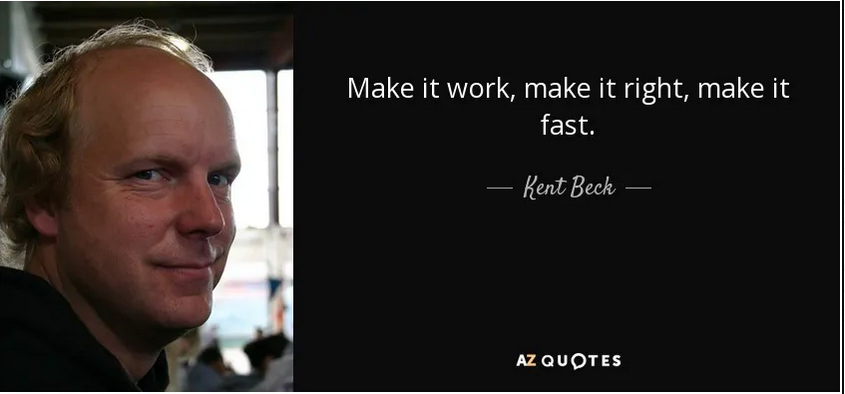
\includegraphics[width=.9\linewidth]{quote.png}
\end{figure}

\end{document}
